\documentclass[letter,12pt]{article}
\usepackage[paperheight=27.94cm,paperwidth=21.59cm,bindingoffset=0in,left=3cm,right=2.0cm, top=3.5cm,bottom=2.5cm, headheight=200pt, headsep=1.0\baselineskip]{geometry}
\usepackage{graphicx,lastpage}
\usepackage{upgreek}
\usepackage{censor}
\usepackage[spanish,es-tabla]{babel}
\usepackage{pdfpages}
\usepackage{tabularx}
\usepackage{graphicx}
\usepackage{adjustbox}
\usepackage{xcolor}
\usepackage{colortbl}
\usepackage{rotating}
\usepackage{multirow}
\usepackage[utf8]{inputenc}
\usepackage{float}
\usepackage{hyperref}
\usepackage{listings}
\lstdefinelanguage{JavaScript}{
  keywords={typeof, new, true, false, catch, function, return, null, catch, switch, var, if, in, while, do, else, case, break},
  keywordstyle=\color{blue}\bfseries,
  ndkeywords={class, export, boolean, throw, implements, import, this},
  ndkeywordstyle=\color{darkgray}\bfseries,
  identifierstyle=\color{black},
  sensitive=false,
  comment=[l]{//},
  morecomment=[s]{/*}{*/},
  commentstyle=\color{gray}\ttfamily,
  stringstyle=\color{red}\ttfamily,
  morestring=[b]',
  morestring=[b]"
}
\lstset{
  language=JavaScript,
  basicstyle=\ttfamily\small,
  keywordstyle=\color{blue},
  commentstyle=\color{gray},
  stringstyle=\color{red},
  numbers=left,
  numberstyle=\tiny\color{gray},
  stepnumber=1,
  numbersep=5pt,
  showspaces=false,
  showstringspaces=false,
  tabsize=2
}

\renewcommand{\tablename}{Tabla}
\usepackage{fancyhdr}
\pagestyle{fancy}


%
\begin{document}
%
   \title{\Huge{Informe Laboratorio 4}}

   \author{\textbf{Sección 1} \\  \\Cristopher Osorio Kappes \\ e-mail: cristopher.osorio\_k@mail.udp.cl}
          
   \date{Mayo de 2024}

   \maketitle
   
   \tableofcontents
 
  \newpage
  

\section{Descripción de actividades}
Para este laboratorio, deberá utilizar Tampermonkey y la librería CryptoJS (con SRI) para lograr obtener los mensajes que le está comunicando su informante. En esta ocasión, su informante fue más osado y se comunicó con usted a través de un sitio web abierto a todo el público https://cripto.tiiny.site/.\par
Sólo un ojo entrenado como el suyo logrará descifrar cuál es el algoritmo de cifrado utilizado y cuál es la contraseña utilizada para lograr obtener la información que está oculta.
\begin{enumerate}
    \item Desarrolle un plugin para tampermonkey que permita obtener la llave para el descifrado de los mensajes ocultos en la página web. La llave debe ser impresa por la consola de su navegador al momento de cargar el sitio web. Utilizar la siguiente estructura:
    \begin{itemize}
        \item   La llave es: KEY
    \end{itemize}
    
    \item En el mismo plugin, se debe detectar el patrón que permite identificar la cantidad de mensajes cifrados. Debe imprimir por la consola la cantidad de mensajes cifrados. Utilizar la siguiente estructura:
    Los mensajes cifrados son: NUMBER
    
    \item En el mismo plugin debe obtener cada mensaje cifrado y descifrarlo. Ambos mensajes deben ser informados por la consola (cifrado espacio descifrado) y además cada mensaje en texto plano debe ser impreso en la página web. \par
    El script desarrollado debe ser capaz de obtener toda la información del sitio web (llave, cantidad de mensajes, mensajes cifrados) sin ningún valor forzado. Para verificar el correcto funcionamiento de su script se utilizará un sitio web con otro texto y una cantidad distinta de mensajes cifrados. Deberá indicar la url donde se podrá descargar su script.\par
    Un ejemplo de lo que se debe visualizar en la consola, al ejecutar automáticamente el script, es lo siguiente:

    \begin{figure}[H]
        \centering
        \includegraphics[width=16cm]{Desarrollo/ejemplo.jpg}
        \label{fig:ejemplo}
    \end{figure}

\end{enumerate}

\section{Desarrollo (Parte 1)}
\subsection{Detecta el cifrado utilizado por el informante}

    \begin{figure}[H]
        \centering
        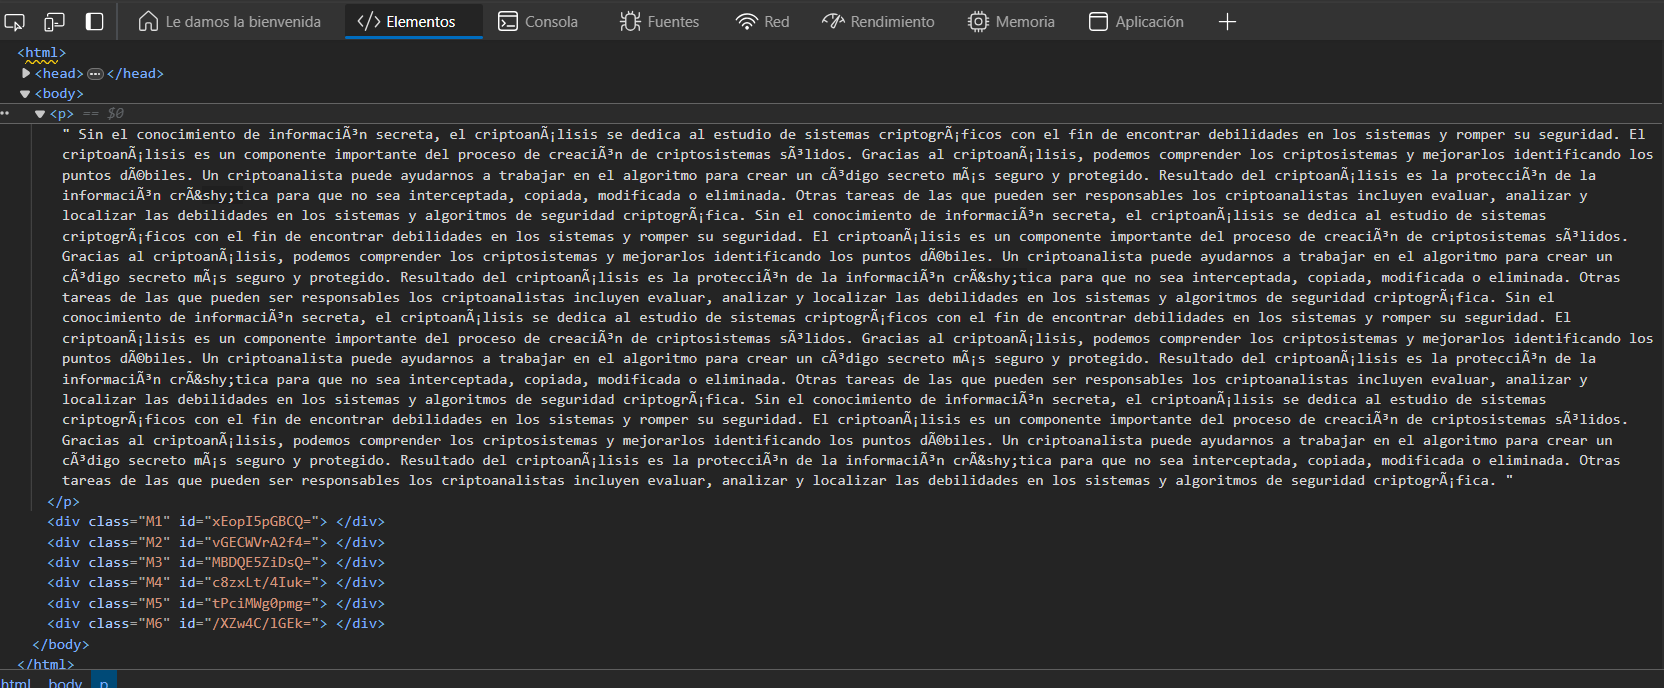
\includegraphics[width=15cm]{img/parte 1/2.1.png}
        \label{fig: 2.1}
        \caption{Vista al inspeccionar la pagina.}
    \end{figure}


Para detectar el cifrado utilizado por el informante, se opta por inspeccionar el sitio web como se puede observar en la imagen \ref{fig: 2.1}, viendo el texto plano entre los ''tags'' ''<p>'' y notando hay 6 lineas con ''tags'' ''<div>'' que contienen una sección ''id'' con textos de 11 caracteres en base 64 con 1 carácter para ''padding'' en cada uno.\newline

En este laboratorio al tener solo una llave para cifrar un mensaje, se puede pensar que se está trabajando con un algoritmo de cifrado simétrico. 


%Al inspeccionar el c´odigo fuente del sitio web, se puede ver que los tags ”div” tiene un ”id” poco com´un: estos est´an en codificaci´on base64. Todos los ”id” de los ”div” se componen de 11 caracteres en base64 y 1 caracter para padding (”=”). Considerando que se tienen mensajes cifrados y una llave a encontrar, se puede decir que se trata de cifrado sim´etrico.


\subsection{Logra que el script solo se gatille en el sitio usado por el informante}

Para que el ''script'' solo pueda usarse en el sitio del informante se agrega la siguiente linea de código:

\begin{lstlisting}
// @match        https://cripto.tiiny.site/*
\end{lstlisting}


\subsection{Define función que obtiene automáticamente el password del documento}

    \begin{figure}[H]
        \centering
        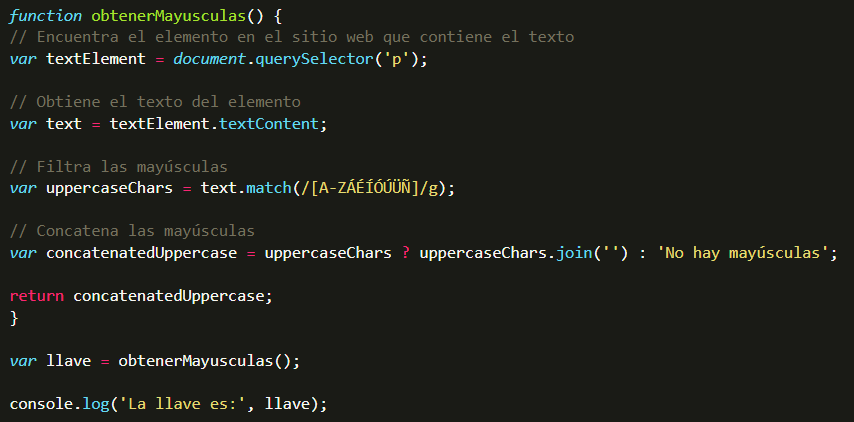
\includegraphics[width=15cm]{img/parte 1/2.3.png}
        \label{fig: 2.3}
        \caption{Función de obtención de password.}
    \end{figure}

La función del código mostrado en la imagen \ref{fig: 2.3} obtiene la llave del sitio web. Se utiliza ''console.log'' para mostrar la llave en consola en el formato pedido. Se debe mencionar que el código finalmente utilizado para este laboratorio no es de 

%La funci´on del C´odigo 2 obtiene autom´aticamente la llave dentro del sitio web y retorna el resultado.

\subsection{Muestra la llave por consola}

    \begin{figure}[H]
        \centering
        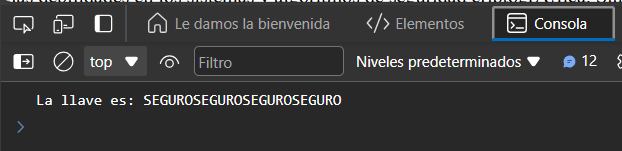
\includegraphics[width=15cm]{img/parte 1/2.4.png}
        \label{fig: 2.4}
        \caption{Obtención de la llave por consola.}
    \end{figure}

En la imagen \ref{fig: 2.4} se puede ver la llave por consola siendo esta: ''SEGUROSEGUROSEGUROSEGURO''.

\section{Desarrollo (Parte 2)}

\subsection{Reconoce automáticamente la cantidad de mensajes cifrados}
    \begin{figure}[H]
        \centering
        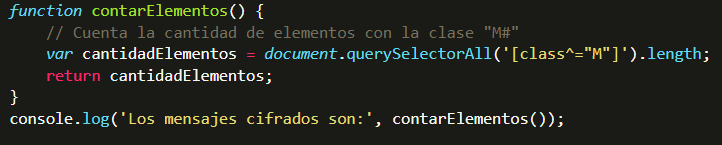
\includegraphics[width=15cm]{img/parte 2/3.1.png}
        \label{fig: 3.1}
        \caption{Función para retornar la cantidad de mensajes cifrados.}
    \end{figure}

La función de la imagen \ref{fig: 3.1} cuenta la cantidad de elementos en donde se tenga la clase ''M'', esto debido a que todos los mensajes cifrados cuentan con ella, tal como se ve en la imagen \ref{fig: 2.1}.

\subsection{Muestra la cantidad de mensajes por consola}
    \begin{figure}[H]
        \centering
        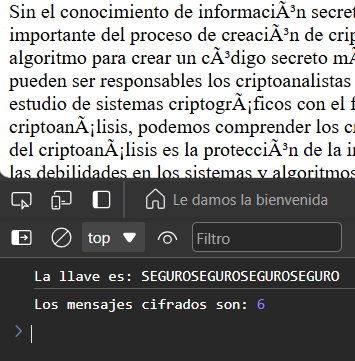
\includegraphics[width=8cm]{img/parte 2/cantidad.png}
        \label{fig: cantidad}
        \caption{Función para obtención de cantidad de mensajes.}
    \end{figure}

La imagen \ref{fig: cantidad} muestra por consola la cantidad de mensajes cifrados del sitio web.

\section{Desarrollo (Parte 3)}

\subsection{Importa la librería cryptoJS}
    \begin{figure}[H]
        \centering
        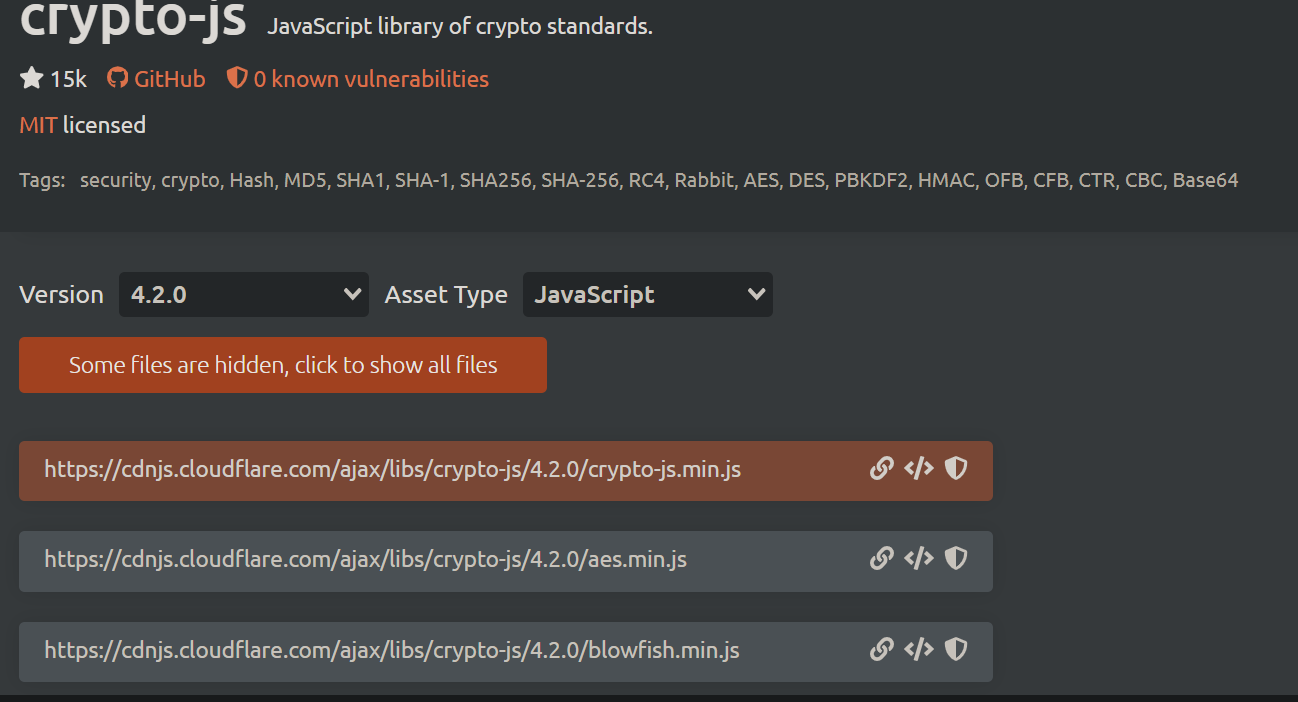
\includegraphics[width=8cm]{img/parte 2/pagina.png}
        \label{fig: pagina}
        \caption{Pagina de donde se extrajo la librería.}
    \end{figure}
    
La librería se obtiene de la pagina del la imagen \ref{fig: pagina}, cuya ''url'' es la siguiente, ''\url{https://cdnjs.com/libraries/crypto-js}''. Se importa ''crypto-js'' copiando la ''url'' correspondiente a ''\url{https://cdnjs.cloudflare.com/ajax/libs/crypto-js/4.2.0/crypto-js.min.js}'' y se agrega a la linea ''@require'' como se muestra a continuación: 
\begin{lstlisting}
// @require https://cdnjs.cloudflare.com/ajax/libs/crypto-js/4.2.0/crypto-js.min.js
\end{lstlisting}



\subsection{Utiliza SRI en la librería CryptoJS}

    \begin{figure}[H]
        \centering
        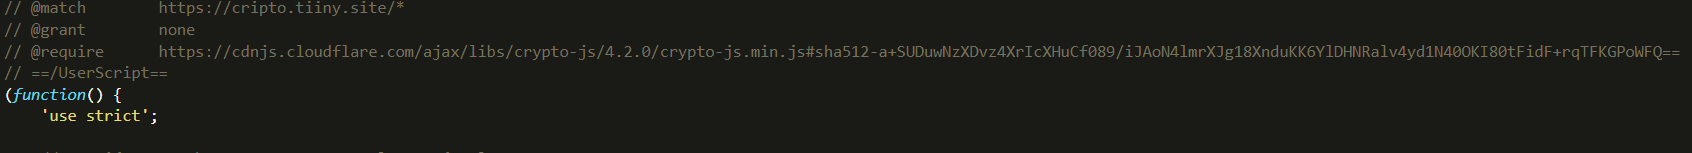
\includegraphics[width=8cm]{img/parte 3/4.2.png}
        \label{fig: 4.2}
        \caption{SRI hash.}
    \end{figure}
    
Se copia de la misma pagina mostrada en la imagen \ref{fig: pagina} la SRI Hash apretando en el simbolo del escudo. Para usarla se agrega al ''@require'' un ''\#'' junto a la librería ''cryptoJs'' para luego agregar el SRI copiado, tal como se ve en la imagen \ref{fig: 4.2}.


\subsection{Repercusiones de SRI inválido}

El ''SRI'' permite verificar a los navegadores si los recursos obtenidos se entregan sin manipulaciones por medio de un ''Has'' criptográfico. Un ''SRI'' inválido es cuando el ''Hash'' de un archivo no coincide con el ''Hash'' del ''HTML'' que carga el recurso. Algunas repercusiones que podría tener el uso de un SRI invalido según la pagina \url{https://dev.to/inchukwudi/understanding-subresource-integrity-sri-3ep7} son:
\begin{itemize}
    \item Bloqueo de recursos al encontrar un hash que no coincide.

    \item Corromper la funcionalidad del sitio web.
\end{itemize}

\subsection{Logra decifrar uno de los mensajes}

Como se trabaja en con solo una llave en un mensaje cifrado se puede asumir que se requiere de un algoritmo de cifrado simétrico, llegando a probar 3DES en modo ECB, el cual permitió obtener un mensaje descifrado legible. Por ejemplo el mensaje descifrado de ''xEopI5pGBCQ='' es : ''este''.


\subsection{Imprime todos los mensajes por consola}

  \begin{figure}[H]
        \centering
        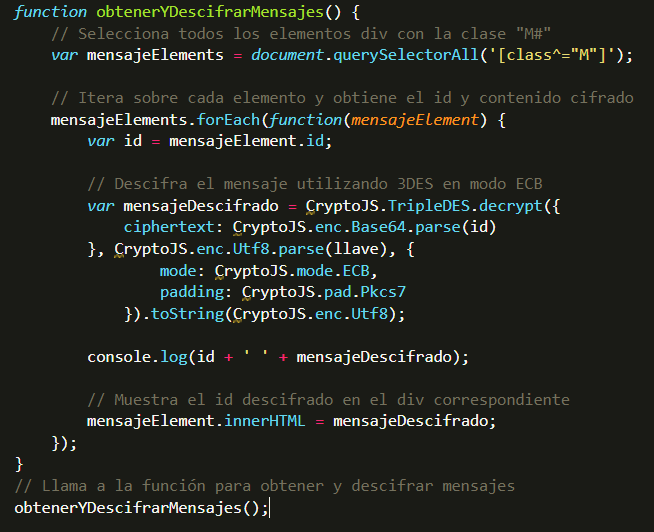
\includegraphics[width=15cm]{img/parte 3/4.5.png}
        \label{fig: 4.5}
        \caption{Función para obtención de mensajes.}
    \end{figure}

En la imagen \ref{fig: 4.5} se ve la función utilizada para obtener los mensajes cifrados indicando que se utilice ''TripleDES''. La función selecciona todos los elementos ''div'' con una clase que comience con "M", descifra los mensajes utilizando el algoritmo 3DES en modo ECB(''CryptoJS.TripleDES.decrypt'')  y muestra el resultado descifrado en el mismo elemento div.

      \begin{figure}[H]
        \centering
        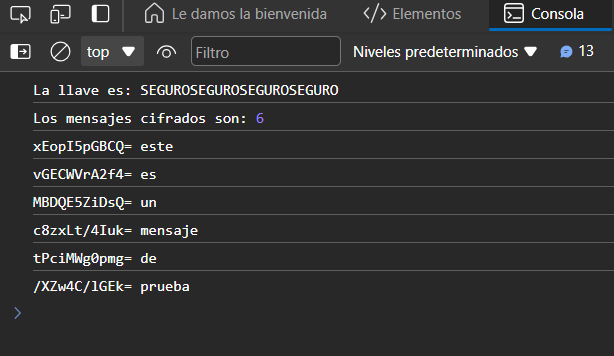
\includegraphics[width=15cm]{img/parte 3/4.5(consola).png}
        \label{fig: 4.6.2}
        \caption{Mensajes mostrados por consola.}
    \end{figure}

En la imagen \ref{fig: 4.6.2} se ven los mensajes descifrados en consola.

\subsection{Muestra los mensajes en texto plano en el sitio web}

  \begin{figure}[H]
        \centering
        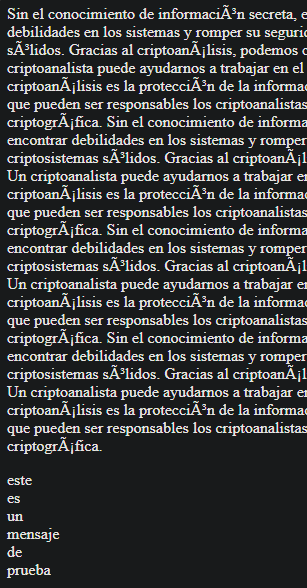
\includegraphics[width=7cm]{img/parte 3/4.6.png}
        \label{fig: 4.6}
        \caption{Obtención de mensajes.}
    \end{figure}

En la imagen \ref{fig: 4.6} se muestran los mensajes directamente en la pagina.
\subsection{El script logra funcionar con otro texto y otra cantidad de mensajes}

\subsection{Indica url al código .js implementado para su validación}



\section*{Conclusiones y comentarios}

\subsection*{Issues}

\end{document}
